\documentclass[a4paper, 12pt]{article}
\usepackage{templates/sbc-template}
\usepackage{color}
\usepackage{graphicx}
\usepackage[brazil]{babel}
\usepackage[utf8]{inputenc}
\usepackage{epsfig}
\usepackage{float}
\usepackage{graphics}
\usepackage{url}
\usepackage[tight,footnotesize]{subfigure}
\usepackage{stfloats}
\usepackage{enumerate}
% \usepackage[left=3cm,top=3cm,right=3cm,bottom=3cm]{geometry}


% correct bad hyphenation here
\hyphenation{op-tical net-works semi-conduc-tor}


\begin{document}

\title{Arquitetura para Mitigação de Ataques DDoS}

\author{
Cinara Menegazzo\inst{1},
Fernando Cezar Bernardelli\inst{1}, \\
Fernando Henrique Gielow\inst{1},
Nadine Lipa Pari\inst{1}
}
   

   
\address{Departamento de Informática -- Universidade Federal do Paraná\\
NR2 - Núcleo de Redes Sem Fio e Redes Avançadas\\
  Caixa Postal 19.081 -- 81.531-980 -- Curitiba -- PR -- Brasil
  \email{\{cmenegazzo,fcb06,fhgielow,nelpari\}@inf.ufpr.br}
}     

\maketitle


\begin{resumo}
%!TEX root = ./proposta3.tex

Ataques de Distributed Denial of Service (DDoS) frequentemente são negligenciados por representarem apenas interrupção de funcionamento normal dos recursos disponíveis. Porém, tratando-se de aplicações destinadas ao comércio eletrônico, uma parada do serviço pode representar grandes perdas financeiras. Com o advento da Internet do Futuro e arquiteturas como a cloud, a mitigação deste tipo de ameaça com o acréscimo de recursos para as aplicações se torna uma alternativa viável, mas que acarreta o problema do economic DDoS. Este artigo apresenta uma proposta de mecanismo para a mitigação de ataques DDoS direcionados a uma aplicação hospedada em uma cloud. Tal mecanismo é baseado na instanciação de uma réplica da aplicação - operação simples em uma cloud - e redirecionamento de apenas requisições legítimas a esta réplica. O mecanismo é inovador por não precisar identificar os clientes atacantes e, ainda assim, conseguir filtrar apenas o tráfego legítimo sem a carga e possíveis erros de categorização que seriam introduzidos pela tentativa de identificação de clientes.

\end{resumo}



\section{Introdução}
%!TEX root = ./proposta3.tex

Diversas pesquisas e propostas têm sido desenvolvidas buscando soluções para problemas da Internet atual, que se propagam para a Internet do Futuro (IF). Tais problemas podem ser amplamente categorizados nas áreas de mobilidade, qualidade de serviço e segurança, os quais ainda caminham para soluções aceitáveis. % expandir o parágrafo com mais uma frase XXXXXXXXXXXXXXXX

Alguns paradigmas mudaram nestas últimas décadas. Hoje, tem-se os dados e aplicações disponibilizados em localizações físicas distintas e desconhecidas. Outra grande mudança ocorreu na forma de administrar um sistema, que antes era de âmbito mais local, com seus usuários e servidores característicos. Agora, tal sistema é hospedado em ambientes construídos pelo compartilhamento de recursos de diversos sistemas autônomos (AS) e heterogêneos.

O uso massivo dos recursos disponibilizados na Internet e toda a conectividade que este ambiente computacional proporciona com serviços para uso pessoal, comercial ou acadêmico, torna este ambiente um alvo visado para códigos maliciosos. Ademais, isso é agravado pela forma como a arquitetura TCP/IP pode favorecer um atacante. O protocolo IP (\emph{Internet Protocol}) omite as informações da verdadeira identidade de um emissor, essa não autenticação da fonte permite ao atacante realizar o ataque contra a vítima, podendo permanecer anônimo e impune. % UMA REFERENCIA AQUI É IMPORTANTE XXXXXXXXXXXXXXXX

Apesar de muitos anos de esforços de pesquisadores, um tipo de ataque ainda representa sérias ameaças a muitos servidores na Internet: o ataque de  \emph{Denial of Service} (DoS). Ele se configura como um dos principais desafios de segurança atualmente propagado para a IF, que interconecta muito mais dispositivos e indivíduos. 


Uma forma de se defender deste tipo de ataque é a prevenção e a reação. O ataque por DoS não visa invadir um computador para obter informações confidenciais, nem tão pouco alterar informações armazenadas nele. Seu objetivo é a indisponibilização de um serviço que está sendo fornecido, utilizando-se do encaminhamento de grandes quantidades de tráfego ao hospedeiro do serviço. Desta forma, este serviço não conseguirá responder a todas as requisições que lhe são encaminhadas. 

O problema se torna ainda mais severo quando diversos geradores de tráfego intensificam o encaminhamento de tráfego de maneira distribuída, caracterizando um ataque de \emph{Distributed Denial of Service} (DDoS \cite{Sachdeva08ddosincidents}). O resultado obtido é o congelamento, a reinicialização, ou ainda o esgotamento completo de recursos necessários ao hospedeiro. Os serviços que mais sofrem com este tipo de ataque são aqueles que permitem requisições anônimas, como serviços web. Assim, o desafio de eliminar os ataques de DDoS está na dificuldade de determinar a diferença entre pacotes legítimos e pacotes de atacantes \cite{Li:2009:DDA:1683304.1684620}.


Com as novas arquiteturas de rede e de aplicações que configuram a IF, surgem sistemas complexos e robustos como \emph{clouds}, onde o desafio de mitigar ataques deste tipo torna-se ainda mais necessário.  Embora o poder de
alocar recursos para suportar um ataque deste tipo  agora torna-se
possível em um \emph{cloud}, crescem com isso também os custos do usuário para manter tais recursos. Tal reação
carateriza o chamado \emph{economic DDoS} (eDDoS \cite{Soon:10}).
  
A maioria das soluções comumente oferecidas para mitigar DDoS em \emph{cloud} se baseiam inteiramente na maior alocação de
recursos \cite{Peng:2007:SND:1216370.1216373}.  %% XXX
%
Algumas abordagens diferenciadas se mostram inadequadas por premissas que nem sempre são verdadeiras ou por serem custosas demais \cite{Bakshi:10}, \cite{Liu:2010:NFD:1866835.1866849}.
%,  colocar mais referencias...... 
Existem diversos registros de ataques que abalaram a Internet nos últimos tempos, como os ocorridos contra o Yahoo!, eBay, Amazon.com e diversos outros \emph{sites} populares em fevereiro de 2000.  No início de 2011 se observou o ataque sofrido pelo hospedeiro de \emph{blogs}, WordPress, que enfrentou o pior ataque de DDoS de sua história \cite{infoexame}.

Ataques deste tipo ainda são disparados em proporções alarmantes, de acordo com descobertas recentes que também revelam a engenharia aplicada que gera redes de zumbis. Um exemplo destas é a rede TDL-4, que é classificada por especialistas em segurança como “não perfeitamente, mas praticamente indestrutível”, com aproximadamente 4,5 milhões de infecções só em 2011 \cite{tdl4}.A partir de fevereiro 2010, o grupo ativista \textit{hacker} conhecido como \textit{Anonymous} começou uma série de ataques de cunho político e ideológico contra várias instituições de porte internacional \cite{titstorm}. A parte mais massiva desses ataques era constituída de DDoS \cite{infoexame}.  Assim, a mitigação de DDoS em \emph{clouds} ainda demanda pesquisas.

O objetivo deste trabalho é elaborar uma arquitetura para mitigação de ataques de
DDoS executados contra uma aplicação hospedada em uma \emph{cloud}. Esta
arquitetura deverá monitorar o tráfego da aplicação e, quando
detectar a possível ocorrência de um ataque de DDoS, criará uma nova
instância desta aplicação, garantindo que nenhum tráfego malicioso a alcance. 


Este trabalho está divido conforme a descrição que segue. Inicialmente,  
a primeira Seção apresenta a introdução do tema. Em seguida, a Seção 2 expõem os trabalhos relacionados, seguido pela arquitetura, na Seção 3. A Seção 4 apresenta uma descrição da implementação que realizaremos. Então, a avaliação a ser realizada é descrita na Seção 5. Por fim, a conclusão é apresentada na Seção 6 e o cronograma na Seção 7.

%estão descritos a motivação e o objetivo deste trabalho, expondo o ambiente de problema e solução que será abordado pela pesquisa. NA seção dois, um levantamento dos trabalhos relacionados é descrito para que se posicione quanto as soluções já existentes. O cenário/arquitetura de .....na seção três

%
%Uma arquitetura de \emph{cloud} pode representar um ambiente propício a ataques por ser usado por diversas pessoas de diversas organizações com suas aplicações e sem o menor controle ou entendimento das configurações ou rede envolvida.
%
%Nos trabalhamos com o targeted attack????
%In a tar-
%geted attack, an adversary wants to gain a critical mass in a
%specific subnet, for example, to attack a specific application
%hosted in that subnet.



\section{Trabalhos Relacionados}
%!TEX root = ./proposta3.tex

A necessidade de proteger ou mitigar as arquiteturas de rede de ataques de DDoS tem sido reconhecida tanto no meio acadêmico quanto comercial. Segundo \cite{1039856}, três são as linhas de defesa contra ataques de DDoS, compreendendo a \textbf{prevenção}, a \textbf{reação}, ou ambas, na chamada defesa \textbf{híbrida}. A prevenção tenta eliminar a possibilidade de ataques de DDoS, isto é, evita a negação de serviço para os clientes legítimos. A linha de reação detecta o ataque e responde imediatamente, e a abordagem híbrida combina os métodos anteriores, não só prevenindo mas também reagindo à ataques.

As pesquisas que envolvem propostas de mitigação de DDoS em arquiteturas de \emph{cloud}, ainda são consideradas incipientes e distantes de uma convergência. Dentre as poucas propostas para estes ambientes, destaca-se o \emph{framework} pró-ativo CluB, apresentado em \cite{Hazelhurst:2008:SCU:1456659.1456671}, que considera uma \emph{cloud} como uma rede constituída de um conjunto de \emph{clusters}, ou \emph{Autonomous Systems} (AS). Estre trabalho sugere
que sejam selecionados determinados roteadores, dispostos de forma distribuída, para análise de tráfego e consequente prevenção de que as requisições maliciosas alcancem a aplicação. Estes roteadores são responsáveis por gerar \emph{tokens} de autenticação para legitimar os pacotes, sendo que a autenticação é necessária para a entrada, saída ou trânsito na arquitetura. Cada \emph{cluster} tem seu código de autenticação, que é trocado periodicamente, podendo ser gerado por uma função \emph{hash}, como MD5 ou SHA. O uso de ferramentas apropriadas de criptografia e atualizações periódicas de componentes da infraestrutura parte da proposta do CluB.



Neste \emph{framework}, todo pacote, malicioso ou não, precisa ser verificado para entrar, sair ou transitar na arquitetura. Cada roteador alocado  deverá realizar a verificação, o que é custoso devido ao \emph{overhead} causado pela autenticação de cada pacote. Também é necessária a implantação e atualização dos algoritmos de análise de tráfego na arquitetura onde estaria sendo utilizado o CluB. Esta questão se torna inviável ao se tratar de uma \emph{cloud}, devido à nebulosidade de sua arquitetura e infraestrutura.

\cite{Verkaik:2006:PCD:1162666.1162673} apresentam outra proposta pró-ativa, que emprega Comunidades de Interesse (COIs) para capturar dados sobre o comportamento coletivo das entidades remotas, utilizando-os para predizer o comportamento futuro. Tal proposta se baseia no fato de que clientes que tiveram relacionamentos legítimos anteriormente possuem bons indícios e podem ser considerados novamente legítimos. Estas afirmações são geradas da observação de comunicações normais da rede e são utilizadas em conjunto com políticas específicas do servidor para mitigar pró-ativamente os ataques de DDoS, usando mecanismos existentes nos roteadores. 
%
Entretanto, a identificação dos clientes passados não é tão trivial. Além do pequeno \emph{overhead} gerado pela verificação, endereços IPs são normalmente dinâmicos e a exigência da realização de \emph{login} para a identificação não é possível, dado que o ataque de DDoS pode a impossibilitar.


Em \cite{Bakshi:10}, ataques são tratados através da criação de uma nova instância da aplicação. Uma vez que um ataque DDoS é detectado, a proposta busca identificar os atacantes através de PINGs: caso um cliente suspeito de ser atacante não responda ao PING, ele é considerado como um atacante, de fato. Desta maneira, apenas os clientes que responderem ao PING serão 
redirecionados para a nova instância da aplicação. Entretanto, tal abordagem depende da premissa que atacantes jamais responderão a PINGs e que clientes genuínos sempre responderão, o que nem sempre condiz com a realidade.



%Filtro de Bloom

\cite{Walfish:2010:DDO:1731060.1731063} apresenta uma forma de mitigação de ataque classificada como defesa baseada em recursos \cite{Dwork:1992:PVP:646757.705669}. %A mitigação emprega o procedimento de que 
Toda vez que um determinado limite de banda é consumido com requisições para um servidor, este servidor, antes que seus recursos se esgotem, encoraja seus clientes a enviar volumes ainda mais altos de tráfego. Considera-se que os atacantes já estariam usando sua capacidade máxima e, assim, eles não poderiam reagir ao encorajamento. A proposta se baseia na premissa que bons clientes tem condições de aumentar seu uso de banda e reagir de forma drástica ao encorajamento. O resultado pretendido é que os bons clientes dominem os maus clientes ao capturar uma fração maior de recursos do servidor. O cliente será atendido caso ele tenha banda o suficiente para se sobressair mediante o tráfego dos atacantes. Um tanto curiosa, esta proposta ocasiona diversos problemas como %a reação apenas quando o servidor já está sendo atacado e o procedimento 
o encorajamento a recebimento de ainda mais tráfego em cenários de ataque. 
% do que o próprio ataque poderia produzir, ou muitas vezes maior, 
Dificilmente um serviço conseguirá atender a tantas requisições e clientes legítimos não necessariamente dominarão o tráfego que chega ao servidor.


Obviamente, a eficácia de todos os esquemas depende criticamente da capacidade de se identificar ou filtrar os clientes legítimos. 
%
WebSoS \cite{Stavrou:2005:WOS:1090583.1648614} é uma adaptação de \emph{Secure Overlay Services} (SOS) \cite{Keromytis:2002:SSO:964725.633032} que mitiga DDoS em servidores web, reativamente após a detecção do ataque. Com uma filtragem robusta de tráfego e bloqueio de requisições~não aprovadas, forma-se um \emph{overlay} seguro. O servidor utiliza mecanismos de autenticação criptográfica e um teste gráfico de Turing \cite{Dietrich00analyzingdistributed} para diferenciar clientes humanos de \emph{scripts} de ataque. Estes procedimentos, segundo os testes dos autores, não sobrecarregam o funcionamento do serviço, porém exigem que os roteadores localizados no perímetro do servidor sejam configurados para controlar o tráfego, procedimento inviável para arquiteturas de \emph{cloud}.

 



\section{Arquitetura para Mitigação de DDoS em \emph{Cloud}}
%!TEX root = ./proposta3.tex


Uma arquitetura em \emph{cloud} envolve a comunicação entre inúmeros componentes através de APIs (\emph{Application Programing Interface}) de serviços web. Os usuários desta arquitetura não sabem e não precisam saber sobre a localização de seus dados ou aplicações que desejem utilizar, porém precisam aceitar e dependem  dos níveis de segurança vigentes, que são tópicos preocupantes para administradores.
A segurança em \emph{cloud} compreende as áreas de segurança de dados e da rede, segundo \cite{Dhage:2011:IDS:1980022.1980076}:  

Enquanto um ataque em dados afeta um número restrito de usuários, um ataque na rede pode comprometer diversos usuários simultaneamente. Como ataques de DDos em uma \emph{cloud} compreendem um ataque à segurança em rede, eles são de importância crítica.  
%Um dos mais importantes fatores para detectar ataques de DDoS é encontrar a correlação entre diferentes fluxos para um mesmo destino.
%
Com a nova infraestrutura de recursos criada pelas \emph{clouds}, existe a possibilidade de se mover fisicamente uma aplicação para outro endereço quando ela é atacada por DDoS. Com isso, é possibilitada a tolerância à falhas e a conservação de recursos despendidos, pois este novo endereço só será conhecido por solicitantes legítimos.

Este trabalho propõe uma arquitetura híbrida para mitigar ataques de DDoS em \emph{clouds} de forma autônoma e independente. Ele se diferencia de outras propostas pela independência da aplicação hospedada, por prover acurácia na filtratem de tráfego legítimo, por não onerar financeiramente o uso dos recursos, e por minimizar os problemas causados pelo ataque sem intervenção humana.
%
A arquitetura proposta poderá ser utilizada por qualquer aplicação hospedada em uma \emph{cloud} que, ao sofrer indícios de um ataque DDoS, filtra o tráfego legítimo e encaminha apenas este para uma nova instância da mesma aplicação. 


\begin{figure}[h!]
\centering
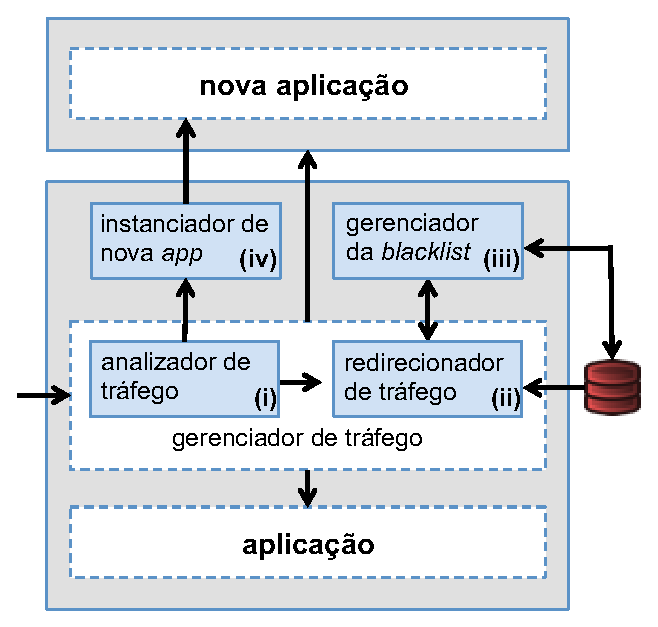
\includegraphics[width=0.55\textwidth]{images/arq.eps}
\caption{Ilustração da proposta de arquitetura para mitigação de ataques DDoS}
\label{fig:arq}
\end{figure}

Esta arquitetura, ilustrada na Figura \ref{fig:arq}, é composta por um módulo geral chamado de Gerenciador de Tráfego (GT), que não se comunica diretamente com a aplicação. Note que a instância do banco de dados é representada exterior às demais instâncias \emph{cloud}, pelo fato de que este banco de dados também está nas nuvens, e pode ser acessado de qualquer outra instância \emph{cloud}. As operações realizadas pelo módulo GT são divididas em quatro submódulos:
% GF virou GT XXXXX


\begin{enumerate}[i]
  \item Analizador de Tráfego (AT);
  \item Redirecionador de Tráfego (RT);
  \item Gerenciador de \emph{Blacklist} (GB);
  \item Instanciador de Nova Aplicação (INA).
\end{enumerate}


O submódulo AT observa o comportamento do tráfego de entrada para a aplicação de forma pró-ativa. Focando-se na estimativa de quantidade de tráfego e de processamento no servidor, este submódulo realiza medição para verificar a existência de um possível ataque DDoS. Caso detectado, o submódulo INA é ativado. O INA criará uma nova instância da aplicação em outro servidor na \emph{cloud}, consequentemente com um endereço IP diferente\footnote{Com a criação da nova instância da aplicação, a antiga é desativada. A primeira instância da \emph{cloud} servirá apenas para redirecionar o tráfego}. Com isso, o submódulo RT passará a tratar todo o tráfego de entrada, respondendo com um redirecionamento para a nova instância da aplicação. Parte-se do princípio que atacantes DDoS não interpretam as respostas obtidas do servidor, pois se interpretarem, sua eficiência é reduzida. Desta maneira, apenas os clientes legítimos serão, de fato, redirecionados à nova aplicação.

Ao redirecionar algum cliente para a nova instância, o endereço deste cliente, seja ele legítimo ou não, será adicionado em uma \emph{blacklist}. Os clientes presentes nesta lista terão suas requisições descartadas, a fim de reduzir o custo de processamento de respostas no servidor. Entretanto, como o cliente legítimo foi informado antes de seu endereço entrar nesta \emph{blacklist}, isso não será um problema, pois ele já terá acesso à nova instância enviando nova requisição. Serão empregadas entradas com tempo de validade nesta \emph{blacklist}, dado que respostas podem ser perdidas. O tempo de validade na lista aumentará exponencialmente, para diminuir ainda mais a sobrecarga. Cabe ao GB, o papel de adicionar e gerenciar a saída de endereços de clientes à \emph{blacklist}, assim como, o tempo de validade da entrada que aumenta exponencialmente.

Contudo, para prevenir que este controle impeça o acesso de clientes legítimos nas próximas requisições, o cliente, ao ser direcionado para a nova instância, terá este endereço armazenado na forma de \emph{cookie} em sua máquina. Este procedimento garante que apenas clientes legítimos tenham conhecimento do novo endereço da aplicação, dado que atacantes de DDoS não irão manter \emph{cookies}. Por fim,  tal processo de reinstanciação de aplicação e redirecionamento de tráfego pode ser repetido recursivamente, até um dado número máximo de redirecionamentos.

A Figura~\ref{fig:cen} ilustra um cenário sob ataque de DDoS, sendo que os clientes são representados pelos ícones dos diversos navegadores, e a nave é o logo da aplicação LOIC (\emph{Low Orbit Ion Cannon}). À esquerda, todos eles enviam seu tráfego para o que imaginam ser a instância da aplicação. Considerando um cenário sob ataque, a aplicação será replicada, e a sua instância original servirá para redirecionar o tráfego legítimo até a aplicação nova. À direita, é ilustrado o resultado do redirecionamento: clientes genuínos conseguem atingir a instância nova da aplicação, enquanto os atacantes mantém o ataque na antiga instância de \emph{cloud}, que agora opera apenas redirecionando tráfego.


\begin{figure}[t!]
	\centering
	\includegraphics[width=0.40\textwidth]{images/an1.eps}
	% \caption{bla}
	\hskip 1cm
	\includegraphics[width=0.40\textwidth]{images/an2.eps}
	\caption{Comportamento do tráfego em um cenário sob ataque}
	\label{fig:cen}
\end{figure}


\section{Implementação}

% \subsection{Detecção de DDoS}
% %!TEX root = ./proposta3.tex


% \subsection{Mecanismo de mitigação}
Para a implementação, inicialmente foram estudadas as possibilidades de serviços \emph{cloud}, como o Amazon, Linode e o Heroku. Dentre estes, o que se apresentou como o mais adequado para a implementação prática de um protótipo operacional de nosso mecanismo foi o Heroku. \cite{heroku} é uma solução em \emph{cloud} que oferece a infra-estrutura como serviço de hospedagem, possibilitando desenvolvimento em frameworks como \emph{django}, \emph{node.js} e \emph{Ruby on Rails}. Dentre estas alternativas, a implementação será realizada em \emph{Ruby on Rails} (RoR), por maior experiência de membros do grupo e pela versatilidade da linguagem, que se mostra mais direta para a implementação, embora qualquer outro \emph{framework} e linguagem pudessem ser utilizados.

A arquitetura do \emph{framework} RoR é completamente baseada no paradigma \emph{Model View Controler} (MVC), facilitando a organização dos módulos de nosso mecanismo. Desta forma, a estrutura do código escrito em RoR é composta de componentes de Modelo, de Visão e de Controle. Componentes de \textbf{modelo} correspondem aos dados - como eles são armazenados, obtidos, correlacionados. A parte de \textbf{visão} corresponde à parte gráfica da aplicação. Finalmente, \textbf{controladores} realizam a manipulação de dados como um todo, correspondem à parte lógica e funcional do código. Eles funcionam também como uma ponte entre modelo e visão, para que os dados transitem em ambos os sentidos.

Desta maneira, o submódulo analizador de tráfego (AT) do nosso mecanismo corresponderá a um controlador. Uma requisição à aplicação será interceptada por esse componente de controle, que realizará a medição de algumas estatísticas e dados, e imediatamente em seguida, acionará o controlador que corresponde ao funcionamento da aplicação em si. Deve-se notar, contudo, que o tempo despendido neste controlador é ínfimo, é apenas o tempo necessário para processar algumas equações e salvar estes dados de controle. Caso se perceba que o tempo afetará o funcionamento do nosso mecanismo, este processamento pode ainda ser realizado em segundo plano.

Caso o AT detecte a existência de um possível ataque, uma nova instância \emph{cloud} deve ser criada pelo submódulo INA e a aplicação replicada para esta, paralisando a aplicação original. O processo de reinstanciação da aplicação pode ser obtido de duas maneiras. A abordagem mais simples seria a pré existência de uma segunda aplicação, sem nenhum recurso alocado. Entretanto, embora esta instância estaria pronta para que seus processos sejam escalados assim que necessário, esta abordagem não se comporta adequadamente no cenário de reinstanciação recursiva. A segunda abordagem envolve a hospedagem do projeto em um repositório do GitHub, que poderá ser clonado para a especificação da segunda instância a partir de dentro do código Ruby. Contudo, esta etapa da implementação ainda requer mais estudos para melhor detalhamento.

Uma particularidade interessante do \emph{framework} RoR é a existência de um arquivo de configuração a cerca das rotas. A implementação do submódulo redirecionador de tráfego (RT) será realizada em cima deste arquivo, chamado \emph{routes.rb}. Para a exibição de qualquer página dinâmica da aplicação, o arquivo de rotas é inevitavelmente chamado. Desta forma, é o local ideal para a adição de clientes na \emph{blacklist} e respectiva filtragem dos clientes bloqueados pelo gerenciador da \emph{blacklist} (GB). No redirecionamento do tráfego para uma nova instância, uma entrada será adicionada, bloqueando o cliente em questão por determinado tempo.

A \emph{blacklist} em si e diversas outras variáveis de controle serão gerenciadas pela base de dados em \emph{cloud}~\cite{redis}. Esta base de dados é famosa pela sua simplicidade e eficiência. Ela basicamente mapeia \textbf{chave} e \textbf{dado}, oferecendo tempos de escrita e leitura correspondentes à \emph{hashing}. Desta forma, uma possibilidade para a implementação da \emph{blacklist} é o uso do Redis, utilizando o IP de um cliente como chave, e o tempo que este cliente permanecerá bloqueado como dado. Por ser, abstratamente, um mecanismo de \emph{hashing}, o tempo de checagem por um cliente será O(1), o que é excelente para um mecanismo que vai filtrar todo tráfego que chega à aplicação.

Por fim, um aspecto interessante do uso do Heroku são os diversos \emph{addons} já customizados para o uso nele. Em particular, existe um \emph{addon} chamado \emph{New Relic} que é designado à coleta de diversas métricas para a análise de desempenho. Com seu uso, será possível saber com precisão o que se passa em todas as instâncias \emph{cloud} de uma perspectiva diretamente interna à esta \emph{cloud}. Assim, poderemos coletar dados não só da perspectiva externa à \emph{cloud}, perspectiva de usuário, como também, de perspectiva interna~à~ela.




\section{Descrição da Avaliação}
%!TEX root = ./proposta3.tex


%A avaliação de um sistema de defesa para ataques pode ser avaliado sobre os aspectos de sua construção. 
% WTF esse trecho acima? xD
%
Uma solução para mitigar ataques pode ser avaliada quanto a sua capacidade de detectar ataque, assim como, a de reagir a ele. Outra abordagem para avaliar uma solução é quanto a sua capacidade de manter as condições normais de funcionamento do cenário de ataque, mesmo sob ataque. Segundo \cite{4600003} é importante para um sistema de defesa estimar diversos aspectos como: custo de desenvolvimento, desempenho, degradação do serviço e custo de robustez. 

A maioria das métricas para calcular o impacto de ataques DDoS estão relacionadas com as medidas de eficiência dos padrões de defesa \cite{4809152}. Atualmente, são consideradas estratégias de medição da quantidade de tráfego legítimo que chega até a aplicação. Outros trabalhos tem se concentrado na medida do tempo de resposta para avaliar a eficiência de uma solução. \cite{Mirkovic:2007:TUM:1281700.1281708} utiliza um modelo baseado em \emph{threshold} como métrica para aferir o impacto de DDoS. Quando uma medida excede este \emph{threshold}, ocorre a  indicação da baixa qualidade do serviço. Esta medida é indicada para aplicações fim-a-fim, como o HTTP.


A etapa de avaliação do nosso mecanismo consistirá principalmente na análise
da capacidade do servidor em atender novas requisições. Se o ataque de DDoS for devidamente
mitigado, as requisições de atacantes serão ignoradas, após a inclusão do requisitante na \emph{blacklist}. Assim, o servidor na \emph{cloud} deverá ser capaz de redirecionar apenas clientes legítimos 
para a nova instância e garantirá que eles terão acesso direto nas próximas requisições. %ISTO CABE A PARTE DE ARQUITETURA.....Com isso, para a análise, serão utilizadas ferramentas que geram requisições ao servidor. Como exemplos, o comando 
%\emph{curl} pode ser utilizado em linha de comando para gerar uma requisição HTTP, sendo necessária a criação de \emph{scripts} mais robustos para incorporar diversas requisições. Outra alternativa é o uso do comando \emph{ab}, que permite a especificação do número de requisições que devem ser realizadas, a concorrência destas requisições, o tempo máximo que se deve esperar por respostas, e diversos outros parâmetros.
Portanto, de acordo com as métricas especificadas por \cite{4600003}, este trabalho de pesquisa fará uso de métricas como o tempo de resposta do servidor para requisições atendidas, a taxa de requisições atendidas com relação ao número de clientes, a carga gerada pelos módulos da arquitetura de acordo com o número de clientes \footnote{O termo ``clientes'', usado neste parágrafo engloba tanto clientes legítimos quanto atacantes.}. 

Cabe ressaltar que este trabalho não necessita de uma previsão muito grande na detecção no sentido de que é melhor realizar uma calibragem muito sensível e possuir falsos positivos do que possuir falsos negativos. Isto ocorre devido à natureza do nosso mecanismo. Se uma nova instância for criada e o trafego for redirecionado à toa, o custo serão alguns mínimos milisegundos de latência. Caso o mecanismo não detecte um ataque, o custo será muito mais significativo. Desta maneira, a avaliação quanto à falsos positivos não será tão necessária. % quanto a avaliação não detecção do ataque. 


\subsection{Cenários}
%!TEX root = ./proposta3.tex

Para a simulação do tráfego necessário, podem ser utilizadas ferramentas que enviam requisições HTTP à aplicação. Como ferramentas, podem ser citados os comandos \emph{curl} e \emph{ab} e a aplicação \emph{LOIC}. A diferença fundamental dentre elas é o nível na qual operam. Enquanto o comando \textbf{curl} opera realizando instâncias singulares de operações simples como \emph{GET}s e \emph{PUT}s, o comando \textbf{ab} automatiza o processo realizando diversas operações de acordo com alguns parâmetros. É possível customizar o nível de concorrência e o intervalo entre as requisições, por exemplo. Tal ferramenta possibilita a medição de algumas métricas como a taxa de entrega de pacotes e o tempo de resposta. Em um nível ainda maior, a aplicação~\cite{loic} foi desenvolvida a fim de realizar ataques de DoS\footnote{Diversos clientes a utilizam a fim de gerar um ataque de DDoS.}. Ela realiza automaticamente a calibragem de diversos parâmetros em níveis inferiores. Entretanto, ela ainda permite a customização de alguns, como a porta de ataque e o protocolo a ser utilizado.

Considerando estas ferramentas, alguns cenários podem ser elaborados para a avaliação. 
%
Para a simulação de clientes legítimos, o comando \emph{curl} pode ser utilizado para criar um \emph{script} que atua como um cliente legítimo. O comando requisitará pela página em questão através de um \emph{GET}. Caso a resposta indique uma mudança de endereço, o \emph{script} será responsável por seguir todas as mudanças e redirecionamentos com chamadas subsequentes do comando \emph{curl}, até que o destino final seja de fato atingido. Deve-se ressaltar que esse comportamento é dificultado em ataques de DDoS, pois eles perderiam muito a sua eficiência ao aguardar por respostas de requisições, para poderem analisar elas, e seguir até o destino final.

Para a obtenção de tempos de resposta e taxa de perda de pacotes da perspectiva do cliente, o comando \emph{ab} pode ser empregado para realizar as medições. Diversas faixas de parâmetros podem ser estipuladas para simular diferentes tipos de comportamentos ou cenários. O uso do \emph{ab} torna-se preferível ao do \emph{curl} quando o objetivo é coletar métricas e não simular um cliente genuíno, afinal, o comando \emph{ab} medirá o desempenho de instâncias \emph{cloud} isoladas, sem realizar qualquer redirecionamento de tráfego. Este aspecto do comportamento do \emph{script} em questão é importante para a diferenciação entre ataques DDoS e \emph{Flash Crowds}~\cite{Thapngam:2011p27061}. Enquanto um ataque é malicioso, uma \emph{Flash Crowd} indica que diversos clientes legítimos estão, de fato, realizando diversas requisições à aplicação. Este caso não será tratado, embora talvez possa ser identificado.

Por fim, para a simulação do ataque DDoS em si, a ferramenta \emph{LOIC} será utilizada, pois ela é uma ferramenta utilizada para ataques reais. Embora a escala em nosso experimento seja muito menor, a operação será baseada em um ataque real e, portanto, condizente com a realidade. Para a obtenção de diferentes endereços IP, diferenciando um DoS de um DDoS, a ferramenta será utilizada simultaneamente por computadores de endereços diferentes.

\section{Conclusão}
%!TEX root = ./proposta3.tex

Este trabalho apresentou uma proposta de arquitetura de mitigação para ataques de DDoS direcionados à aplicações web hospedadas em \emph{cloud}. A arquitetura é dependente apenas da existência do ambiente na \emph{cloud}. Os quatro sub módulos especificados garantem o funcionamento das etapas de forma autônoma até mesmo para gerar uma nova instância da aplicação. Assim como permitirá livre acesso para os clientes legítimos, dado que apenas eles realizarão o redirecionamento solicitado. O uso da \emph{blacklist} terá gerencimento eficiente pelo uso de tempo de validade, que no caso de atacantes, terá aumento exponencial para reincidências.




\section{Cronograma}
%!TEX root = ./proposta3.tex

O desenvolvimento deste trabalho de pesquisa segue as etapas descritas no cronograma descrito abaixo, onde '$\circ$' define as atividades já realizadas e '$\bullet$' as atividades a serem desenvolvidas 
{\footnotesize
\center
\begin{table}[ht!]
\footnotesize
\center
\begin{tabular}{|c||c|c|c|c|c|c|c|}
\hline

      & \textbf{Nov/1} & \textbf{Nov/2} & \textbf{Nov/3} & \textbf{Nov/4} & \textbf{Dez/1} & \textbf{Dez/2} & \textbf{Dez/3} \\
\hline
\hline
Elaboração da proposta de solução      &  {$\circ$} & {$\circ$} &  &  &  &  &  \\
\hline						
%&  {\color{green}$\bullet$} & {\color{green}$\bullet$} &  &  &  &  &  \\
Estudo de métricas de desempenho      &  & {$\circ$} & $\bullet$ &  &  & &  \\
\hline									

Pesquisa sobre detecção de DDoS      &  & {$\circ$} & $\bullet$  &  &  &  &  \\
\hline									


Pesquisa sobre ferramentas       &  &  & {$\circ$} &  &  &  &  \\
para geração de requisições       &   &   &   &   &   &   &   \\
\hline									


Implementação dos módulos      &  &  &  {$\circ$} & $\bullet$ & $\bullet$ & $\bullet$ &  \\
\hline									

Escrita do relatório final      &  &   & {$\circ$} & $\bullet$  & $\bullet$ &  $\bullet$ &  \\
\hline

Experimentação      &  &  &  &  &$\bullet$  & $\bullet$ &  \\
\hline
\end{tabular}
\label{tab:crono}
\end{table}
}


\section{Acknowledment}
%!TEX root = ./proposta3.tex

Este trabalho foi realizado mediante a colaboração de todos os membros da equipe, onde o problema a ser tratado e o escopo de solução foram discutidos por todos e todos tiveram participação. As etapas descritas no cronograma tiveram a seguinte divisão de trabalho, embora a participação de todos seja essencial e deva ser mantida para que o trabalho tenha um todo como resultado e não apenas partes de esforços.


\begin{itemize}
\item Elaboração da proposta de solução - Todos
\item Estudo de métricas de desempenho - Cinara e Fernando Gielow
\item Pesquisa sobre detecção de DDoS - Cinara
\item Pesquisa sobre ferramentas para geração de requisições - Fernando Cezar
\item Implementação dos módulos - Fernando Gielow e Fernando Cezar
\begin{itemize}
\item Especificação de Algoritmos - Cinara e Nadine com suporte de todos
\item Estudo de ferramentas - Fernando Gielow e Fernando Cezar
\end{itemize}
\item Escrita do relatório final - Cinara e Nadine
\item Experimentação - Todos
\begin{itemize}
\item Categorização e medição de métricas - Cinara e Fernando Gielow
\end{itemize}

\end{itemize}





% \newpage
% \bibliographystyle{unsrt}

\bibliographystyle{templates/sbc}
\bibliography{parts/proposta3}
\end{document}
